\documentclass[10pt,a4paper,oneside]{article}

%-----------------------------------------------------------------------
% Packages
\usepackage[utf8]{inputenc}
\usepackage[italian]{babel}
\usepackage{amsmath}
\usepackage{amsfonts}
\usepackage{amssymb}
\usepackage{graphicx}
\usepackage{lmodern}
\usepackage[colorlinks]{hyperref}

%-----------------------------------------------------------------------
% Package configuration
\hypersetup{
 urlcolor = blue
}

%-----------------------------------------------------------------------
% Heading
\title{Specifica progetto}
\author{Programmazione a oggetti}

%-----------------------------------------------------------------------
% Document
\begin{document}
\maketitle

%-----------------------------------------------------------------------
\section{Introduzione}
Lo scopo del progetto è lo sviluppo in C++ di un'applicazione a tema libero soggetta a vincoli obbligatori dotata di un'interfaccia grafica (GUI) realizzata mediante il framework \href{https://www.qt.io/?hsLang=en}{Qt}. Il progetto potrà essere sviluppato da un singolo studente oppure da una coppia di studenti e dovrà richiedere approssimativamente 50 ore di lavoro complessivo individuale.

La GUI può liberamente trarre ispirazione sia da applicazioni per sistemi desktop che app per sistemi mobile. Si potrà aderire ai \emph{design pattern} \emph{Model-View-Controller} o \emph{Model-View} per la progettazione architetturale della GUI. Qt include un insieme di classi \emph{view} che usano una architettura \emph{Model/View} per gestire la relazione tra i dati logici della GUI ed il modo in cui essi sono presentati all'utente della GUI. Il framework Qt è dotato di una documentazione completa e precisa che sarà la principale guida di riferimento nello sviluppo della GUI, oltre ad offrire l'IDE QtCreator ed il tool QtDesigner. L'applicazione potrà anche applicare \emph{design pattern} comunemente utilizzati in C++.

I voti relativi alla prova scritta e al progetto sono tra loro indipendenti e il voto finale sarà calcolato come la loro media pesata. È possibile riconsegnare il progetto mantenendo il voto della prova scritta (e viceversa). È possibile sostenere la prova scritta senza aver consegnato il progetto e viceversa, tuttavia la valutazione di quest'ultimo con relativo feedback avverrà solamente dopo aver superato l'esame scritto. Affinché un progetto possa essere valuto valutato deve essere consegnato durante la finestra relativa alla sessione in cui si intende verbalizzare il voto; questa regola si applica anche a progetti già valutati e senza modifiche (in questo caso riconsegnare una copia del progetto precedentemente consegnato).

%-----------------------------------------------------------------------
\section{Roadmap}
\begin{center}
 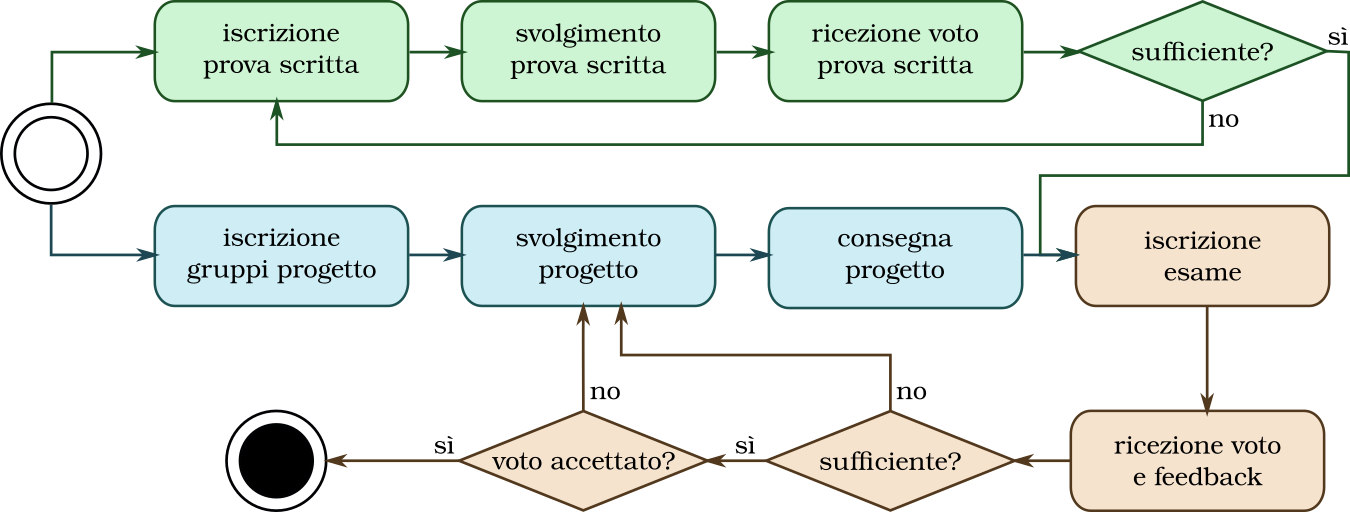
\includegraphics[width=0.85\textwidth]{assets/roadmap}
\end{center}

%-----------------------------------------------------------------------
\section{Iscrizione e gruppi}
È possibile svolgere il progetto singolarmente o in gruppi di due studenti. In ogni caso \textbf{è necessario registrarsi compilando il Google Form} all'indirizzo \url{https://forms.gle/wJCah6iCbX5j5R517} entro le 23:59 del 15 gennaio 2023 (Europe/Rome).


%-----------------------------------------------------------------------
\section{Vincoli}
Il progetto deve obbligatoriamente soddisfare i seguenti vincoli:
\begin{enumerate}
 \item essere un \textbf{lavoro originale} dello studente o del gruppo di studenti
 \item essere interamente \textbf{scritto in C++}
 \item prevedere un'\textbf{interfaccia grafica} realizzata in Qt
 \item \textbf{compilare senza errori} sulla macchina virtuale fornita (sono tollerati, sebbene generalmente penalizzati, i \emph{warning} durante la compilazione)
 \item implementare una \textbf{gerarchia di classi} con almeno tre classi concrete per i progetti svolti singolarmente, o almeno cinque classi concrete per i progetti svolti in gruppo
 \item consentire la \textbf{creazione, la modifica e la cancellazione} degli oggetti della gerarchia
 \item implementare nativamente almeno un \textbf{contenitore per oggetti della gerarchia}, il quale dovrà esporre almeno un metodo per l'inserimento, uno per la lettura, uno per la cancellazione e uno per la ricerca in base a qualche criterio; a titolo esemplificativo e non esaustivo un contenitore può essere una lista singolarmente collegata, doppiamente collegata, una blockchain, un insieme o un albero; tali metodi dovranno essere effettivamente utilizzati all'interno del programma, benché non sia necessario che ciò avvenga tramite la GUI (per es. inserimento nel contenitore durante la lettura da file); il contenitore deve essere utilizzato in almeno un punto del programma, ma è possibile utilizzare anche altre strutture dati, come \emph{std::vector}, in parti diverse del programma
 \item realizzare la \textbf{persistenza dei dati} in una qualsiasi forma per i progetti svolti singolarmente, o in un formato strutturato (JSON, XML, \ldots) per i progetti svolti in gruppo
 \item mantenere una \textbf{separazione netta} tra il modello logico e l'interfaccia grafica, ovvero il codice del modello deve poter essere riutilizzabile senza dipendere dall'interfaccia; nulla vieta che il codice del modello utilizzi strumenti di Qt non legati all'interfaccia, come le funzioni di I/O o le classi per la gestione di JSON
 \item realizzare i principi di \textbf{incapsulamento e \emph{information hiding}} della programmazione a oggetti: una classe deve astrarre un singolo concetto e includere tutti gli attributi e metodi di cui ha bisogno con opportuni livelli di visibilità
 \item utilizzare il \textbf{polimorfismo in maniera non banale}; alcuni esempi di utilizzo \emph{banale} sono i distruttori virtuali, metodi \emph{getter} che restituiscono informazioni leggermente diverse a seconda dell'oggetto di invocazione, metodi \emph{getType} che restituiscono una stringa contenente il tipo dell'oggetto; per contro un utilizzo \emph{non banale} del polimorfismo si può ottenere con metodi che svolgono operazioni diverse a seconda del tipo concreto dell'oggetto, come costruire un \emph{widget} grafico diverso a seconda dell'oggetto da mostrare; molti \emph{design pattern} richiedono un utilizzo del polimorfismo non banale e possono pertanto fornire ottimi spunti
 \item eseguire in maniera \textbf{efficiente e robusta}, senza errori a \emph{runtime}
 \item essere corredato di una \textbf{relazione}, in lingua italiana o inglese, di massimo 8 pagine con testo a 10pt che riporti:
 \begin{enumerate}
  \item nome, cognome e numero di matricola di tutti i componenti del gruppo (o del singolo autore in caso di progetto svolto singolarmente)
  \item una breve introduzione che spieghi il tema scelto
  \item la descrizione del modello logico
  \item la descrizione dell'utilizzo non banale del polimorfismo
  \item la descrizione del metodo utilizzato per la persistenza dei dati
  \item la descrizione delle funzionalità implementate
  \item la rendicontazione delle ore previste e di quelle effettivamente svolte
  \item solo per progetti svolti in gruppo: la suddivisione delle attività
  \item solo per progetti riconsegnati: una sezione che riporta le modifiche apportate; in caso di riconsegna senza modifiche è preferibile aggiungere comunque questa sezione indicando che non ci sono state modifiche
 \end{enumerate}
 In caso di progetto di gruppo, le relazioni devono essere distinte. Assieme al documento di specifiche viene fornito anche un modello commentato di relazione il cui utilizzo non è obbligatorio. Si suggerisce inoltre l'uso di \href{https://it.wikipedia.org/wiki/LaTeX}{LaTeX}, il sistema di scrittura universalmente usato dagli informatici in ambito accademico.
\end{enumerate}

%-----------------------------------------------------------------------
\section{Consegna}
La consegna avverrà tramite il Moodle del corso, all'interno del quale saranno attivate cinque sessioni di consegna del progetto per gli altrettanti appelli d'esame previsti. Si dovrà consegnare un unico archivio in formato zip della dimensione massima di 256MB attraverso l'apposita pagina Moodle. \textbf{Non saranno accettati tentativi di consegna con modalità diverse o formati che non siano zip}. La cartella compressa dovrà contenere:
\begin{itemize}
 \item la relazione in formato PDF
 \item una sottocartella con i file sorgente del progetto (.h, .cpp, .pro, eventuali sottocartelle) ed eventuali file multimediali necessari (immagini, icone, ecc.)
 \item almeno un file d'esempio per la persistenza dei dati
\end{itemize}
La cartella \emph{non dovrebbe} contenere codice oggetto compilato, eseguibili, file generati dall'IDE o in generale qualsiasi file non sia utile ai fini della valutazione. Si raccomanda di verificare il corretto caricamento dei file su Moodle e di comunicare tempestivamente eventuali malfunzionamenti.

In caso di progetti di gruppo ogni studente dovrà provvedere alla consegna includendo il codice (lo stesso per tutti i membri del gruppo) e la propria relazione (diversa per ciascuno). Se nel gruppo solamente uno studente è sufficiente all'esame scritto, questo studente può comunque procedere alla consegna del progetto con l'obiettivo di finalizzare l'esame. Si ricorda che la valutazione del progetto con relativo feedback avverrà solamente per gli studenti sufficienti all'esame scritto e che abbiano effettuato la consegna nella sessione in cui intendono registrare il voto.


%-----------------------------------------------------------------------
\section{Criteri di valutazione}
Il progetto viene valutato sulla base dei vincoli obbligatori e delle funzionalità implementate. Più precisamente, \textbf{se uno o più vincoli obbligatori non risultano soddisfatti il progetto verrà considerato insufficiente} e sarà necessaria una riconsegna in uno degli appelli successivi. Viceversa, \textbf{se tutti i vincoli obbligatori sono soddisfatti il progetto è considerato (almeno) sufficiente} e la valutazione aumenterà in base alla qualità delle funzionalità sviluppate e, in misura minore, in base alla qualità della relazione.

Una funzionalità viene valutata positivamente in base alla sua pertinenza al tema scelto, all'utilità, all'usabilità, alla complessità e alla qualità del codice attraverso cui è implementata. Funzionalità più semplici o generiche migliorano la valutazione, sebbene non tanto quanto idee più complesse o articolate. Le scorciatoie da tastiera, per esempio, sono migliorie generiche semplici da ottenere con poche righe di codice in Qt, così come la gestione del ridimensionamento delle finestre o l'uso di icone. Per contro l'integrazione con un sistema di API o l'uso di basi di dati come SQL o MongoDB per la persistenza sono significativamente più complessi e richiedono la scrittura di classi apposite.

La qualità della relazione, pur avendo un'incidenza minore, verrà valutata sulla base della completezza della chiarezza e della coesione. \textbf{Errori linguistici evidenti} come sistematica mancanza di punteggiatura o errori di battitura frequenti \textbf{verranno penalizzati}. È possibile redigere la relazione in Italiano o Inglese, a propria discrezione. La scelta della lingua non avrà effetti sulla valutazione.

Poiché il corso non tratta di usabilità o resa estetica della GUI la loro mancanza \textbf{non verrà penalizzata}, purché questo non pregiudichi il corretto funzionamento del programma. Tuttavia, se il progetto viene svilupatto ponendo attenzione a questi temi, verrà riconosciuto un bonus come se si trattasse di una funzionalità aggiuntiva.

La valutazione del progetto è \textbf{valida per l'intero anno accademico} e fino a che non viene (ri)consegnato un progetto. La valutazione è accompagnata da un feedback testuale che motiva il voto proposto e sottolinea i punti di forza e debolezza del progetto.

È possibile riconsegnare un progetto per ottenere una nuova valutazione, la quale potrà essere peggiorativa, tuttavia se si seguono le indicazioni del feedback sarà generalmente migliorativa. La valutazione è \emph{idempotente}: riconsegnare lo stesso progetto senza modifiche produrrà esattamente lo stesso voto.

Consegnare un progetto svolto da altri (con o senza il loro consenso) comporta automaticamente l'insufficienza.

La registrazione del voto finale è possibile solo dopo:
\begin{itemize}
 \item avere superato con valutazione maggiore o uguale a 18 la prova scritta
 \item essersi iscritti alla lista Uniweb della per la registrazione del voto finale
 \item avere consegnato il progetto entro la scadenza prevista per la sessione in cui si intende verbalizzare il voto e aver ottenuto una valutazione positiva
\end{itemize}
Il giorno della registrazione del voto verrà inviato all'email istituzionale dei soli studenti iscritti alla lista uniweb di registrazione del voto finale il feedback relativo alla valutazione del progetto e verrà comunicato il voto finale complessivo dell'esame. In caso di valutazione negativa del progetto, l'esame non sarà superato: sarà quindi necessaria la riconsegna del progetto per una successiva scadenza di consegna; in questo caso il voto dell'esame scritto rimane comunque valido. Lo studente che rifiuterà il voto finale proposto via uniweb dovrà riconsegnare il progetto per una successiva scadenza di consegna (tranne all'ultimo appello d'esame), cercando quindi di porre rimedio ai punti deboli segnalati nel feedback di valutazione e descrivendo obbligatoriamente le modifiche apportare al progetto nella relazione aggiornata; anche in questo caso il voto sufficiente dell'esame scritto rimane comunque valido. Il voto finale verrà calcolato come media pesata delle valutazioni ottenute nella prova scritta e nel progetto.

%-----------------------------------------------------------------------
\section{Note}
I video-tutorati dell'anno accademico 2020/2021 del tutor Benedetto Cosentino dedicati all'apprendimento delle caratteristiche di base del framework Qt per la progettazione di GUI sono disponibili su \href{https://www.youtube.com/playlist?list=PLH_Fd-836q-VcqWnnzsq3GOF2-0i_Az7p}{YouTube}.

\end{document}